\documentclass{article}
\usepackage[preprint]{neurips_2026}
\usepackage[utf8]{inputenc}
\usepackage[T1]{fontenc}
\usepackage{amsmath,amssymb}
\usepackage{graphicx}
\usepackage{booktabs}
\usepackage{multirow}
\usepackage{hyperref}
\usepackage{xcolor}
\usepackage{enumitem}
\usepackage{caption}
\usepackage{subcaption}
\usepackage{natbib}
\usepackage{wrapfig}
\bibliographystyle{plainnat}

\newcommand{\ours}{\textsc{SandboxDR}}

\title{\ours{}: A Reproducible Multi-Source Benchmark\\for Deep Research Agents with Deterministic Ground Truth}

\author{Anonymous Authors}

\begin{document}
\maketitle

% ======================================================================
\begin{abstract}
Deep research agents have proliferated since 2025. These systems decompose complex queries, search heterogeneous sources, and synthesize long-form cited reports~\citep{drsurvey2025}. Evaluation, however, remains fragmented. The dominant paradigm of live-web benchmarking conflates agent capability with retrieval infrastructure, produces non-reproducible results, and cannot detect citation fabrication~\citep{browsecomp_plus2025,liu2023verifiability}. We introduce \ours{}, a fully reproducible benchmark infrastructure of 100 cross-source research tasks spanning 13 domains and 6 intent types (recommendation, comparison, debunking, causal explanation, timeline, enumeration); evaluation in this paper covers a 30-task common subset across 9 open-source frameworks, with an extension to 56 tasks for the rank-1 agent as a stability check. Agents search, interact with, and synthesize information from three containerized sandbox sources: an e-commerce storefront, a discussion forum, and an encyclopedia. All agents face an identical, frozen retrieval surface. Each task carries a curated ground truth of $\geq$120 must-cite URLs and a 21-item evaluation checklist. We observe a \emph{text-quality--only ranking inversion}: against a no-gate quality composite that omits citation truthfulness, an agent that fabricates 97.5\% of its citations rises from rank~5 to rank~1 (Kendall $\tau{=}0.50$). The inversion attenuates substantially ($\tau{=}0.91$) when the no-gate baseline includes citation alignment, suggesting that the failure mode is specifically text-and-URL-syntax-only scoring rather than no-gate scoring per se. Combining this with an adversarial URL-stuffing attack analysis, we argue that deterministic citation verification (existence + quotation) plus an LLM-judged claim-source alignment dimension are jointly necessary for sound deep research assessment, and that LLM-judge evaluation~\citep{llmjudge2024} alone cannot detect the failure modes we surface.
\end{abstract}

% ======================================================================
\section{Introduction}
\label{sec:intro}

Deep research is the process by which an agentic AI system decomposes a complex, open-ended query into sub-tasks, iteratively retrieves evidence from diverse sources, and synthesizes the results into a structured, citation-grounded report~\citep{draco2026,drbench2026}. Unlike closed-book question answering~\citep{gaia2024,hle2025} or single-hop retrieval-augmented generation~\citep{frames2024,fanoutqa2024}, deep research demands multi-step planning, cross-source reasoning, and the production of long-form outputs whose breadth rivals that of a human domain expert~\citep{drsurvey2025}.

Both commercial and open-source deep research systems have multiplied rapidly. Commercial offerings (OpenAI Deep Research, Gemini Deep Research, and Perplexity Deep Research) now serve millions of queries daily. Open-source frameworks such as STORM~\citep{storm2024}, Co-STORM~\citep{costorm2024}, MindSearch~\citep{mindsearch2025}, GPT-Researcher~\citep{gptresearcher2024}, and CAMEL-AI~\citep{camelai2023} have made deep research accessible to the broader community. This proliferation has created a pressing need for standardized evaluation.

\paragraph{The reproducibility crisis.} The benchmark landscape has grown correspondingly: DRACO~\citep{draco2026}, DR.~Bench~\citep{drbench2026}, LiveResearchBench~\citep{liveresearchbench2026}, ResearchRubrics~\citep{researchrubrics2025}, DeepResearch Bench~\citep{drb2025}, and others~\citep{drb2_2026,mmdr2026,dr9k2026,reportbench2025,kdrbench2026} have collectively proposed thousands of evaluation tasks. However, nearly all rely on live-web APIs. As \citet{browsecomp_plus2025} observe, such evaluations ``conflate agent system performance with the effectiveness of their retrieval components, [which] severely undermines the reproducibility of experiments.'' The same agent, run on the same benchmark one month apart, may produce different results simply because search rankings have shifted, websites have been updated, or API rate limits have changed~\citep{deepresearchgym2025}. This makes controlled scientific comparison impossible.

\paragraph{The citation truthfulness gap.} A subtler but equally serious problem is \emph{citation fabrication}. Deep research agents are expected to cite their sources, yet we find that some agents generate fluent, well-structured reports with high LLM-judge scores while fabricating the vast majority of their citations. The phenomenon has antecedents in the citation-faithfulness literature: \citet{liu2023verifiability} measure citation precision and recall on commercial generative search engines and document substantial gaps between fluency and groundedness; FActScore~\citep{factscore2023} and SAFE~\citep{safe2024} extend the analysis to atomic-fact-level evaluation; \citet{citeme2024} examine citation accuracy for scientific claims; \citet{maynez2020faithfulness} situate the broader faithfulness-vs-fluency tradeoff in abstractive summarization. Existing DR benchmarks, which evaluate reports primarily through text-quality rubrics~\citep{draco2026,liveresearchbench2026,researchrubrics2025}, do not verify whether a cited URL actually exists, let alone whether it supports the claim made in the report. Our contribution is an empirical operationalization of this concern in the agentic-DR setting: we exploit a frozen sandbox to make citation-existence verification deterministic and zero-cost, surface a ranking-inversion phenomenon under text-only scoring, and quantify its sensitivity to the specific weighting choices.

\paragraph{Contributions.} We present \ours{}, a benchmark designed to address both gaps simultaneously:
\begin{enumerate}[leftmargin=*,itemsep=3pt]
\item \textbf{Three-source interactive sandbox} (\S\ref{sec:sandbox}). We combine a Magento e-commerce storefront (${\sim}2{,}000$ products), a Postmill discussion forum (${\sim}5{,}000$ threads), and a Kiwix-served English Wikipedia mirror (${\sim}200{,}000$ articles) into a single Docker-based environment. Unlike prior sandboxes that offer either pure IR~\citep{deepresearchgym2025,browsecomp_plus2025} or pure task completion~\citep{webarena2024}, ours requires agents to exercise both retrieval and interaction across heterogeneous source types.

\item \textbf{100-task corpus with an intent-type taxonomy} (\S\ref{sec:tasks}). Tasks span 13 domains and 6 intent types (Recommendation, Comparison, Debunking, Causal, Timeline, Enumeration), enabling stratified analysis that flat, untyped benchmarks cannot support. The empirical leaderboard in this paper (\S\ref{sec:experiments}) is computed on a 30-task common subset, with an extension to 56 tasks for the rank-1 agent as a stability check; the remaining 70 tasks have golden URL sets and checklists generated and validated and are released alongside the corpus.

\item \textbf{Curated citation ground truth with deterministic verification} (\S\ref{sec:golden}). Each task is paired with $\geq$120 must-cite sandbox URLs (mean 135) and a 21-item checklist. Existence and verbatim quotation are checked deterministically against the frozen sandbox; claim-source alignment is checked by an LLM judge in the ALCE-attribution paradigm~\citep{alce2023}.

\item \textbf{Text-only ranking inversion and its sensitivity} (\S\ref{sec:f6}). Removing our URL-reachability gate causes the most citation-fabricating agent to rank first under a text-only quality composite (Kendall $\tau{=}0.50$). Crucially, the inversion attenuates to $\tau{=}0.91$ when the no-gate baseline is allowed to include citation alignment, isolating which scoring choices the failure mode is and is not sensitive to. We further show the V3 composite is gameable by a synthetic URL-stuffer adversary and recommend complementary defenses.
\end{enumerate}

% ======================================================================
\section{Related Work}
\label{sec:related}

We organize prior work along two axes: how agents access information (live-web vs.\ controlled), and how outputs are scored.

\paragraph{Live-web DR benchmarks.} DeepResearch Bench~\citep{drb2025} pioneered PhD-level evaluation across 22 fields, later extended with rubric-based diagnostics in DRB~II~\citep{drb2_2026}. DRACO~\citep{draco2026} raised the bar with 100 tasks mined from Perplexity production queries, graded by 26 domain experts across 4 axes and ${\sim}39$ rubric criteria per task. LiveResearchBench~\citep{liveresearchbench2026} evaluates 17 systems on 100 dynamic tasks, while ResearchRubrics~\citep{researchrubrics2025} provides expert-crafted rubrics for 101 tasks across 9 domains. DR.~Bench~\citep{drbench2026} covers 214 tasks with a multiplicative composite incorporating semantic drift. The landscape continues to expand: MMDeepResearch-Bench~\citep{mmdr2026} targets multimodal report generation (140 tasks, 21 domains), DeepResearch-9K~\citep{dr9k2026} scales to 9{,}000 questions, ReportBench~\citep{reportbench2025} benchmarks against expert academic surveys, and KDR-Bench~\citep{kdrbench2026} emphasizes structured-knowledge grounding with 1{,}252 tables. Across these benchmarks, the same limitation recurs: live-web dependence makes exact replication impossible.

\paragraph{Controlled-environment benchmarks.} Recognizing this, several works have moved toward static or sandboxed corpora. BrowseComp~\citep{browsecomp2025} proposed 1{,}266 fact-seeking questions; BrowseComp-Plus~\citep{browsecomp_plus2025} froze these into a 100K-document corpus, cleanly demonstrating that retrieval quality alone accounts for a 14-point gap on GPT-5. DeepResearchGym~\citep{deepresearchgym2025} indexes ClueWeb22 and FineWeb via DiskANN, achieving sub-commercial-API latency. DR$^3$-Eval~\citep{dr3eval2026} constructs per-task static corpora with multimodal support. On the interactive side, DRBench Enterprise~\citep{drbench_ent2026} containerizes four enterprise applications in Docker. WebArena~\citep{webarena2024} pioneered multi-app sandboxing for web agents but targets task completion, not research synthesis.

\paragraph{Evaluation methodology.} Beyond output quality, TRACE~\citep{trace2026} evaluates trajectory efficiency and cognitive quality at the ACM Web Conference 2026. IDRBench~\citep{idrbench2026} benchmarks interactive DR with user-in-the-loop feedback. For citation evaluation specifically, ALCE~\citep{alce2023} establishes the claim-source alignment paradigm under static corpora. \citet{llmjudge2024} survey LLM-as-judge methods and document position bias, verbosity bias, and self-enhancement bias. Bradley-Terry paired-comparison Elo, as we use here for leaderboard construction, has been popularized for LLM evaluation by Chatbot Arena~\citep{chatbot_arena2024}.

\paragraph{Citation faithfulness lineage.} The ``fluent but ungrounded'' failure mode we surface in \S\ref{sec:f6} has antecedents.  \citet{maynez2020faithfulness} formalize the faithfulness-vs-fluency tradeoff in abstractive summarization. \citet{liu2023verifiability} measure citation precision and recall on commercial generative search engines, finding fluent outputs with substantial citation gaps. FActScore~\citep{factscore2023} and SAFE~\citep{safe2024} extend the analysis to atomic-fact-level evaluation. FacTool~\citep{chern2023factool} pipelines factuality detection across modalities. \citet{citeme2024} target citation accuracy for scientific claims specifically. Our contribution relative to this lineage is empirical, not conceptual: we operationalize citation-existence verification as a deterministic, zero-cost, complete check by running it inside a frozen sandbox, and we quantify the size and weighting-sensitivity of the resulting ranking effect on agentic-DR systems.

\paragraph{Agent frameworks.} STORM~\citep{storm2024} generates Wikipedia-like articles via outline-first, multi-perspective questioning; Co-STORM~\citep{costorm2024} extends this to collaborative human-agent dialogue. MindSearch~\citep{mindsearch2025} mimics human cognitive search with a DAG-based multi-agent architecture. \citet{drsurvey2025} provide a taxonomy distinguishing plan-and-execute, iterative-refinement, and multi-agent paradigms.

\paragraph{Our positioning.} Table~\ref{tab:comparison} situates \ours{} within this landscape. We inherit WebArena's~\citep{webarena2024} interactive sandbox lineage and BrowseComp-Plus's~\citep{browsecomp_plus2025} static-corpus reproducibility, and add two features absent from all prior benchmarks: intent-type stratification and deterministic citation ground truth.

\begin{table}[t]
\centering
\caption{Comparison with representative deep research benchmarks. \textbf{Reprod.}~= reproducible across time; \textbf{M-src}~= heterogeneous multi-source; \textbf{Inter.}~= interactive sites (not pure IR); \textbf{Intent}~= structured intent taxonomy; \textbf{Cite-GT}~= ground truth at the citation level (must-cite URL set per task); \textbf{Task-GT}~= deterministic task-completion check (e.g., programmatic state). \ours{} contributes Cite-GT where most prior DR benchmarks lack any citation-level ground truth; WebArena and DRBench-E contribute Task-GT (functional checks) which we do not provide.}
\label{tab:comparison}
\vspace{1mm}
\small
\setlength{\tabcolsep}{4pt}
\begin{tabular}{@{}lcccccccc@{}}
\toprule
\textbf{Benchmark} & \textbf{Tasks} & \textbf{Dom.} & \textbf{Reprod.} & \textbf{M-src} & \textbf{Inter.} & \textbf{Intent} & \textbf{Cite-GT} & \textbf{Task-GT} \\
\midrule
DRACO~\citep{draco2026}               & 100 & 10 & \texttimes & \texttimes & \texttimes & \texttimes & rubric only & \texttimes \\
LiveResBench~\citep{liveresearchbench2026}   & 100 & 7  & \texttimes & \texttimes & \texttimes & \texttimes & rubric only & \texttimes \\
DR.~Bench~\citep{drbench2026}         & 214 & 10 & \texttimes & \texttimes & \texttimes & \texttimes & rubric only & \texttimes \\
ResRubrics~\citep{researchrubrics2025} & 101 & 9  & \texttimes & \texttimes & \texttimes & \texttimes & rubric only & \texttimes \\
DRB~II~\citep{drb2_2026}              & 132 & 22 & \texttimes & \texttimes & \texttimes & \texttimes & rubric only & \texttimes \\
ReportBench~\citep{reportbench2025}    & var & acad & \texttimes & \texttimes & \texttimes & \texttimes & rubric only & \texttimes \\
\cmidrule(lr){1-9}
BC-Plus~\citep{browsecomp_plus2025}    & 830 & broad & \checkmark & \texttimes & \texttimes & \texttimes & answer-fact & \texttimes \\
DRGym~\citep{deepresearchgym2025}      & ${\sim}$1K & broad & \checkmark & \texttimes & \texttimes & \texttimes & rubric only & \texttimes \\
DR$^3$-Eval~\citep{dr3eval2026}       & var & multi & \checkmark & \texttimes & \texttimes & \texttimes & rubric only & \texttimes \\
DRBench-E~\citep{drbench_ent2026}     & 100 & ent  & \checkmark & \checkmark & \checkmark & \texttimes & 114 facts & \checkmark \\
WebArena~\citep{webarena2024}          & 812 & web  & \checkmark & \checkmark & \checkmark & \texttimes & \texttimes & \checkmark \\
\midrule
\textbf{\ours{} (Ours)} & \textbf{100} & \textbf{13} & \checkmark & \checkmark & \checkmark & \checkmark & \textbf{must-cite + ALCE} & \texttimes \\
\bottomrule
\end{tabular}
\end{table}

% ======================================================================
\section{Benchmark Design}
\label{sec:design}

\subsection{Sandbox Architecture}
\label{sec:sandbox}

\begin{figure}[t]
\centering
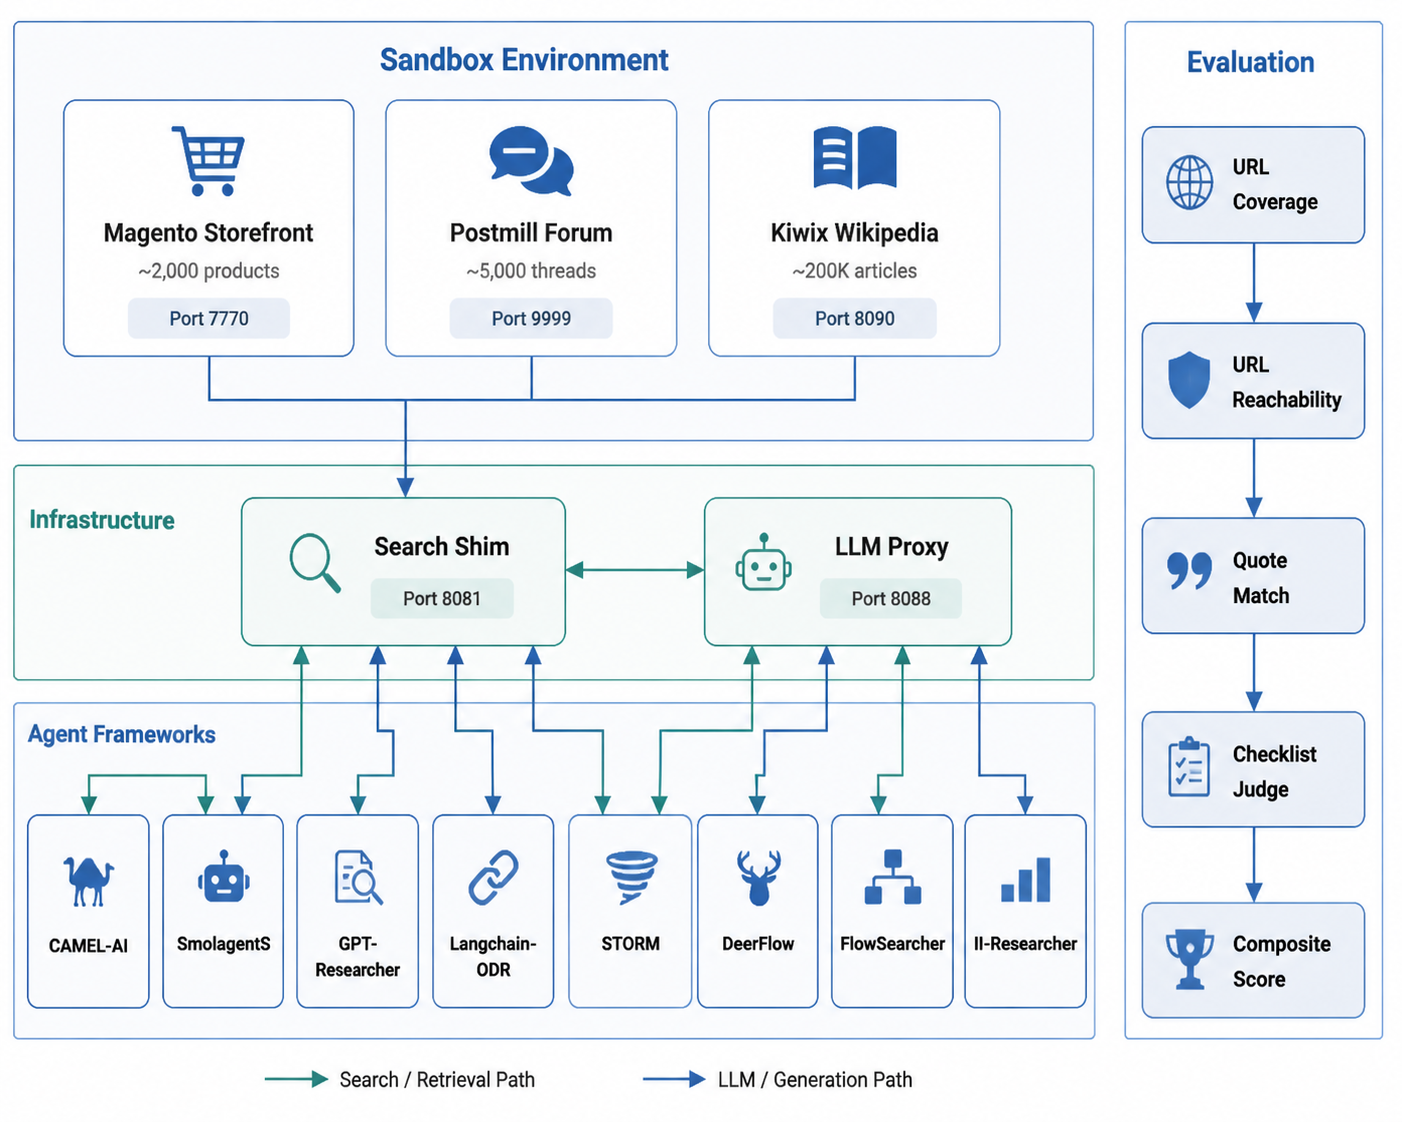
\includegraphics[width=\textwidth]{fig_architecture.png}
\caption{\ours{} architecture. Three Docker-containerized sandbox sources (top) expose heterogeneous information modalities: e-commerce product pages, community discussion threads, and encyclopedic articles. A Tavily-compatible search shim and a centralized LLM proxy (middle) allow unmodified agent frameworks (bottom) to operate without code changes. The evaluation pipeline (right) combines deterministic URL verification with LLM-judge assessment.}
\label{fig:architecture}
\end{figure}

The sandbox (Figure~\ref{fig:architecture}) runs three Docker containers, each serving a distinct information modality:

\textbf{Shopping} (Magento~2, port 7770). Inherited from WebArena~\citep{webarena2024}, the storefront hosts ${\sim}2{,}000$ product pages across categories such as electronics, household goods, books, health products, and outdoor gear. Each product page exposes structured attributes (price, star rating, review count, and free-text feature descriptions) that agents can extract through search or direct browsing.

\textbf{Forum} (Postmill, port 9999). Also from the WebArena ecosystem, the forum hosts ${\sim}5{,}000$ discussion threads across 20+ topic-specific sub-forums (technology, personalfinance, AskReddit, Fitness, etc.). Threads carry metadata including vote scores and comment counts, enabling sentiment analysis.

\textbf{Encyclopedia} (Kiwix, port 8090). An offline Wikipedia mirror serving ${\sim}200{,}000$ articles in the ZIM format. Agents can perform keyword search and read full article text, providing factual and technical grounding.

\textbf{Infrastructure.} A \emph{search shim} (port 8081) presents a Tavily-compatible search API and routes queries to the appropriate sandbox source. All agents share a single LLM backbone, DeepSeek~V4~flash (snapshot date pinned in the supplementary manifest) with chain-of-thought reasoning disabled, accessed through a centralized proxy (port 8088). The agent framework itself is therefore the only experimental variable: architecture, prompting strategy, and tool-use patterns. Reproducibility manifest with image digests, ZIM-file SHA-256, Magento DB snapshot hash, search-shim version, and judge model snapshot date is provided in Appendix~\ref{sec:repro}.

\subsection{Task Design}
\label{sec:tasks}

\paragraph{Scale and domains.} We construct 100 research tasks spanning 13 thematic domains (Table~\ref{tab:domain_intent}). This matches the scale of leading benchmarks: DRACO~\citep{draco2026} and LiveResearchBench~\citep{liveresearchbench2026} each have 100 tasks; ResearchRubrics~\citep{researchrubrics2025} has 101. Our domain coverage (13 domains) exceeds most competitors.

\begin{table}[t]
\centering
\caption{Task distribution across domains and intent types. Each cell shows the number of tasks. The design ensures balanced coverage: 15--17 tasks per intent type and 5--12 per domain.}
\label{tab:domain_intent}
\vspace{1mm}
\footnotesize
\setlength{\tabcolsep}{3pt}
\begin{tabular}{@{}lcccccc|c@{}}
\toprule
\textbf{Domain} & \textbf{Recom.} & \textbf{Comp.} & \textbf{Debunk} & \textbf{Causal} & \textbf{Time.} & \textbf{Enum.} & \textbf{Total} \\
\midrule
Consumer         & 3 & 2 & -- & 1 & 1 & 1 & 8 \\
Health/Medicine  & 2 & 2 & 2 & 2 & 2 & 1 & 11 \\
Technology       & 2 & 2 & 2 & 2 & 2 & 2 & 12 \\
Environment      & 2 & 1 & 2 & 2 & 2 & 2 & 11 \\
Business         & 2 & 1 & 1 & 2 & 1 & 2 & 9 \\
Politics         & 1 & 2 & 1 & 2 & 1 & 1 & 8 \\
Finance          & 1 & 1 & 1 & 1 & 1 & 1 & 6 \\
Law              & -- & 1 & -- & 1 & 1 & 2 & 5 \\
Travel           & 1 & 2 & 1 & -- & 1 & 1 & 6 \\
Education        & 1 & 1 & 1 & 1 & 1 & 1 & 6 \\
Entertainment    & 1 & 1 & 1 & 1 & 1 & 1 & 6 \\
Science          & -- & 1 & 1 & 1 & 1 & 1 & 5 \\
Health/Safety    & 1 & -- & 4 & -- & 1 & 1 & 7 \\
\midrule
\textbf{Total}   & \textbf{17} & \textbf{17} & \textbf{17} & \textbf{16} & \textbf{16} & \textbf{17} & \textbf{100} \\
\bottomrule
\end{tabular}
\end{table}

\paragraph{Intent taxonomy.} Unlike prior benchmarks that treat all tasks as undifferentiated research queries, we introduce a six-type intent taxonomy reflecting distinct cognitive demands:

\begin{itemize}[leftmargin=*,itemsep=2pt]
\item \textbf{Recommendation} (e.g., ``What are the best home blood pressure monitors?''): product search, feature comparison, and sentiment aggregation across shopping and forum sources.
\item \textbf{Comparison} (e.g., ``AWS vs.\ Azure vs.\ GCP for startup workloads''): structured multi-dimensional matrices with evidence from all three sources.
\item \textbf{Debunking} (e.g., ``Audit 5 claims about 5G health risks''): claim extraction, evidence retrieval, and verdict classification (supported/refuted/unclear).
\item \textbf{Causal} (e.g., ``Why do antibiotics cause bacterial resistance?''): causal-chain construction from encyclopedic knowledge, supported by product data and community discussion.
\item \textbf{Timeline} (e.g., ``Evolution of smartphone processors 2007--2026''): chronological organization with dated milestones and citations.
\item \textbf{Enumeration} (e.g., ``Catalog of USB standards and connector types''): exhaustive coverage with structured attributes per item.
\end{itemize}

This taxonomy enables \emph{intent-stratified analysis}: we can identify which agent architectures excel at which cognitive strategies. DRACO~\citep{draco2026}, LiveResearchBench~\citep{liveresearchbench2026}, and all other benchmarks we surveyed lack this capability.

\paragraph{Task generation pipeline.} Tasks are produced through a four-stage semi-automated pipeline:

\textit{Stage 1: Topic generation.} An LLM (GLM-4-flash) proposes candidate topics with domain-specific shopping keywords ($n{=}9$), forum names ($n{=}8$), and Wikipedia article titles (10 mandatory + 15 supplementary). We generate 5 candidates per (domain, intent) cell and select the most sandbox-compatible.

\textit{Stage 2: Sandbox validation.} Every keyword and article title is validated against the live sandbox through HTTP probes: shopping keywords must return $>$0 products, forums must exist in Postmill, and Wikipedia titles must resolve in Kiwix. Invalid entries are replaced with verified alternatives.

\textit{Stage 3: Golden scraping.} A dedicated scraper harvests all relevant URLs from the sandbox for each topic, adaptively balancing across the three sources to produce a golden set of $\geq$120 must-cite URLs (mean: 135, median: 135). Cross-source requirements ensure each golden set spans at least 2 (typically 3) domains.

\textit{Stage 4: Task specification.} An LLM generates the full intent prompt (mean 1{,}937 characters) and a 21-item evaluation checklist tailored to the topic and intent type. Prompts include sandbox placeholders (\texttt{\_\_SHOPPING\_\_}, \texttt{\_\_REDDIT\_\_}, \texttt{\_\_WIKIPEDIA\_\_}) that are resolved at runtime.

\textit{Quality assurance.} All 100 tasks pass automated validation: no missing fields, no unresolved placeholders, golden completeness $\geq$90 must-cite URLs per task, and checklist length $\geq$15 items.

\subsection{Deterministic Ground Truth}
\label{sec:golden}

A key limitation of live-web benchmarks is the absence of stable ground truth~\citep{browsecomp_plus2025}. When an agent cites a URL, the benchmark cannot verify whether that URL existed when the agent ran, what content it contained, or whether it supports the agent's claim. Rubric-based evaluation~\citep{draco2026,researchrubrics2025} partially addresses this through expert-designed criteria, but remains fundamentally text-centric.

\ours{} provides \emph{citation-level} ground truth with \emph{deterministic existence and quotation} verification. For each task, the golden JSON contains: (i) $\geq$120 must-cite URLs drawn from the sandbox (mean 135), representing pages a comprehensive report \emph{should} reference; (ii) a pool of ${\sim}500$ expected URLs representing the broader relevant surface; and (iii) structured knowledge triples (subject, predicate, object, source\_url) extracted from product pages, forum threads, and encyclopedia articles. Because adaptive scraping is used to balance coverage across the three sources (\S\ref{sec:tasks}, Stage 3), the must-cite set should be read as a \emph{sufficient} reference set (an agent that cites these URLs is grounded in the sandbox), not the unique \emph{correct} reference set; multiple defensible reference choices can yield similar coverage.

Because the sandbox is frozen, every URL is stable. We can deterministically check whether a cited URL (a)~exists, (b)~returns HTTP~200, and (c)~contains text matching the agent's quoted excerpt; the fourth criterion --- (d)~whether the cited page \emph{supports} the agent's claim --- is checked by an LLM judge in the ALCE attribution paradigm~\citep{alce2023}, and is therefore not deterministic. We adapt ALCE rather than implement it verbatim: we use citation alignment (judge-rated) as one weighted dimension, and we add a multiplicative reachability gate that ALCE does not have.

\subsection{Scoring Framework}
\label{sec:scoring}

We combine deterministic verification with LLM-judge evaluation across seven weighted quality dimensions plus a truthfulness gate.

\textbf{URL Coverage} ($w{=}0.20$). Must-cite recall (fraction of golden URLs cited), pool coverage, and domain balance across the three sources. This measures coverage: did the agent find the relevant information?

\textbf{URL Reachability} (truthfulness gate, multiplicative). Every cited URL is probed via HTTP. If an agent fabricates URLs, its reachability approaches zero, which multiplicatively floors the composite at 10\% of quality. Treating truthfulness as a near-prerequisite rather than a weighted factor is the central design choice of our scoring framework.

\textbf{Quote Match} ($w{=}0.20$). Fuzzy string matching of in-text quotations against the actual page content at cited URLs, measuring \emph{faithfulness} of extraction.

\textbf{Checklist Judge} ($w{=}0.20$). A 21-item task-specific checklist evaluated by an LLM judge (PASS / FAIL / UNCLEAR per item), following the binary-rubric approach of DRACO~\citep{draco2026}.

\textbf{Spec Compliance} ($w{=}0.10$). Format requirements: word count (3{,}500--8{,}000), citation count ($\geq$60 markdown links), paragraph count ($\geq$25).

\textbf{Citation Alignment} ($w{=}0.15$). For each (claim, cited URL) pair, an LLM judge decides whether the cited page actually supports the claim, following the ALCE paradigm~\citep{alce2023}.

\textbf{Analysis Depth} ($w{=}0.10$). Six structural and six judge-rated criteria capturing causal reasoning, multi-perspective treatment, and quantitative grounding.

\textbf{Presentation} ($w{=}0.05$). Six deterministic format checks plus six judge-rated criteria on clarity and structure.

\paragraph{Composite score.} The truthfulness-gated composite (\textsc{V3}) is:
\begin{equation}
\text{score} = \underbrace{\max(\phi, r)}_{\text{ground gate}} \;\times\; \underbrace{\bigl(0.20\,u + 0.20\,q + 0.20\,j + 0.15\,a + 0.10\,d + 0.10\,s + 0.05\,p\bigr)}_{\text{quality}}
\label{eq:composite}
\end{equation}
where $r{=}\text{reachability}$, $u{=}\text{url\_coverage}$, $q{=}\text{quote\_match}$, $j{=}\text{judge\_pass\_rate}$, $a{=}\text{citation\_alignment}$, $d{=}\text{analysis\_depth}$, $s{=}\text{spec\_compliance}$, $p{=}\text{presentation}$, and $\phi{=}0.1$ is the gate floor. The multiplicative gate floors at $\phi$ to retain partial credit for low-but-nonzero reachability while still penalizing wholesale fabrication: an agent with $r{=}0$ keeps only 10\% of its quality score, an order of magnitude below grounded competitors. We sweep $\phi \in \{0.0, 0.05, 0.1, 0.2, 0.5\}$ in \S\ref{sec:ablation} to expose its sensitivity. We also report two no-gate baselines used in \S\ref{sec:f6} to characterize the fluent-hallucinator phenomenon: \textsc{V1}, an additive ``text-only'' composite $0.4\,u + 0.4\,j + 0.2\,s$ that omits all citation-aware terms ($r$, $q$, $a$); and \textsc{V1$'$}, the same quality vector as the V3 numerator but without the reachability gate (i.e.\ $\max(\phi,r)$ replaced by $1$). The contrast between V1 and V1$'$ is precisely the contribution of citation-aware quality terms to no-gate ranking. Rankings are computed via the Bradley-Terry model~\citep{bradleyterry1952,chatbot_arena2024} fit by MM-iteration with weak Bayesian smoothing (pseudo-count 0.5 to handle agents with no wins) and rescaled to Elo ($1000$ anchor, mean-centered, scale $400/\ln 10$); 95\% CIs come from 1{,}000 bootstrap resamples over tasks.

\paragraph{Dimensions prototyped and dropped.} An additional NLI-based claim-entailment verifier (\texttt{claim\_nli}) was prototyped during scoring development. Under the DeepSeek V4 flash judge with the entailment-threshold prompt we used, support rates were near-zero for all 10 candidate frameworks (per-agent variance $\sigma \approx 0$), making the dimension non-discriminative. We retained it in score files for transparency but assigned it weight zero in \eqref{eq:composite}; future work with stronger entailment models~\citep{alce2023} may reintroduce it.

% ======================================================================
\section{Experiments}
\label{sec:experiments}

\subsection{Systems Evaluated}

We evaluate 9 open-source frameworks, with all LLM calls routed through a centralized proxy to DeepSeek V4 flash (reasoning disabled). The local hardware (NVIDIA RTX~5090, 32\,GB VRAM) hosts the sandbox containers, the search shim, and the LLM proxy; agent computation itself is API-call-bound. The 9 frameworks are:

\begin{itemize}[leftmargin=*,itemsep=1pt]
\item \textbf{CAMEL-AI}~\citep{camelai2023}: Multi-agent role-playing with autonomous tool use.
\item \textbf{SmolagentS}: Hugging Face's code-based agentic framework.
\item \textbf{GPT-Researcher}~\citep{gptresearcher2024}: Parallel sub-query decomposition with iterative report refinement.
\item \textbf{Langchain-ODR}: LangChain's plan-and-execute Open Deep Research.
\item \textbf{STORM}~\citep{storm2024}: Outline-first, multi-perspective questioning.
\item \textbf{DeerFlow}: ByteDance's multi-agent research framework.
\item \textbf{FlowSearcher}: Our hierarchical-memory agent (L1/L2/L3 memory tiers).
\item \textbf{II-Researcher}: Iterative self-critique and refinement.
\item \textbf{Local-Deep-Research} (LDR): Lightweight local-first agent that streams citations as it browses.
\end{itemize}

A tenth framework (\texttt{qx-agents}) was attempted but produces empty reports under our search shim and is excluded from the leaderboard. STORM produces consistently empty (${\le}20$ byte) outputs under the sandbox shim, an integration issue we discuss in \S\ref{sec:errors}; it is retained in the leaderboard for completeness but readers should treat its results as a framework-integration baseline rather than a capability assessment.

Each agent's search is routed to the sandbox shim, and LLM calls go through the shared proxy; no agent has internet access. The judge LLM is the same DeepSeek V4 flash served through a separate endpoint. \emph{We acknowledge a same-family judge configuration:} agent backbone and judge are drawn from the same model family, which the LLM-as-judge survey~\citep{llmjudge2024} flags as a setup susceptible to self-enhancement bias of the order $5$--$10$ Elo points in prior work. Our principal claims (\S\ref{sec:f6}) hinge on \emph{deterministic} URL reachability rather than on judge-rated dimensions, so this bias should not affect the headline ranking-inversion result, but it does affect citation\_alignment, checklist, analysis\_depth, and presentation. A cross-family judge robustness slice (GPT-5-chat vs. DeepSeek on a top-tier-vs-fabricator contrast) is included in the supplementary release; we summarize the agreement statistics in \S\ref{sec:limitations}.

\subsection{Main Results}

\begin{table}[t]
\centering
\caption{Headline leaderboard under the V3 truthfulness-gated composite (Eq.~\ref{eq:composite}, $\phi{=}0.1$). Bradley-Terry Elo (1000-anchor, mean-centered, scale $400/\ln 10$) fit by MM-iteration with weak Bayesian smoothing (pseudo-count 0.5 to keep zero-win agents identifiable); 95\% CIs from 1{,}000 percentile bootstrap resamples over 1{,}080 head-to-head battles ($\binom{9}{2}=36$ pairs $\times$ 30 common tasks). All 9 agents are restricted to the symmetric 30-task common subset for the headline; the n=56 CAMEL-AI extension (\S\ref{sec:limitations}) is reported as an appendix sensitivity check, not in this table. The top~3 form a clear tier separated from the rest by ${>}300$ Elo points; bottom~6 spread is partly driven by framework-integration issues (\S\ref{sec:errors}, particularly STORM and II-Researcher).}
\label{tab:leaderboard}
\vspace{1mm}
\small
\begin{tabular}{@{}rlccccc@{}}
\toprule
\textbf{Rank} & \textbf{Agent} & \textbf{V3 Elo} & \textbf{95\% CI} & \textbf{W} & \textbf{L} & \textbf{D} \\
\midrule
1 & CAMEL-AI            & \textbf{1565} & [1497, 1654] & 222 & 18 & 0 \\
2 & FlowSearcher (ours) & \underline{1463} & [1403, 1543] & 207 & 33 & 0 \\
3 & SmolagentS          & 1343 & [1267, 1439] & 188 & 52 & 0 \\
\cmidrule(lr){1-7}
4 & GPT-Researcher      &  978 & [\phantom{0}920, 1032] & 122 & 118 & 0 \\
5 & Langchain-ODR       &  849 & [\phantom{0}791, \phantom{0}901] &  93 & 147 & 0 \\
6 & DeerFlow            &  840 & [\phantom{0}779, \phantom{0}894] &  91 & 149 & 0 \\
7 & LDR                 &  832 & [\phantom{0}773, \phantom{0}883] &  88 & 150 & 2 \\
8 & II-Researcher       &  641 & [\phantom{0}566, \phantom{0}697] &  46 & 192 & 2 \\
9 & STORM               &  489 & [\phantom{0}396, \phantom{0}555] &  19 & 217 & 4 \\
\bottomrule
\end{tabular}
\end{table}

Table~\ref{tab:leaderboard} presents the primary ranking. CAMEL-AI, FlowSearcher, and SmolagentS form a top tier separated from the rest by ${>}365$ Elo, with non-overlapping 95\% bootstrap CIs against rank-4. The bottom six split roughly into a fabricator cluster (GPT-Researcher, Langchain-ODR) and a low-output cluster (LDR, II-Researcher, STORM).

\paragraph{What separates the tiers?} Table~\ref{tab:profiles} decomposes the composite into its constituent dimensions. The top-3 agents achieve high URL reachability (CAMEL-AI 0.90, FlowSearcher 0.80, SmolagentS 0.71), meaning they actually navigate the sandbox and cite real pages. The bottom six split into two failure modes: \emph{wholesale fabrication} (GPT-Researcher 0.03, Langchain-ODR 0.004, II-Researcher 0.002, STORM 0.0 reachability), and \emph{output collapse} (LDR cites only 67 URLs across 30 tasks; STORM emits empty reports). The fabricators generate plausible-looking sandbox URLs that do not correspond to any page that actually exists.

This failure is decoupled from report quality. GPT-Researcher achieves the highest scores on url\_coverage (0.191), checklist judge (0.610), analysis depth (0.301), and presentation (0.682), outperforming the top tier on three of the seven quality dimensions. Yet its composite score is 0.030, because the truthfulness gate reduces its effective score to 10\% of its quality and its citation\_alignment score is 0.

\paragraph{Per-intent stratified results.} Table~\ref{tab:intent} reports V3 means stratified by intent type, the analysis the intent taxonomy was designed to enable. CAMEL-AI dominates 6 of 7 intent types (Causal, Comparison, Debunking, Enumeration, Market-Intelligence, Recommendation) with V3 means in 0.41--0.49; FlowSearcher (ours) wins on Timeline (0.408 vs CAMEL 0.299), where its hierarchical memory advantage at chronological organization shows up. SmolagentS sits a tier below the top-2 across all intent types except Recommendation. The bottom 5 are below 0.05 on every intent.

\begin{table}[t]
\centering
\caption{V3 composite mean stratified by intent type, on the symmetric $n{=}30$ common subset. ``$n$'' is the number of tasks in each intent cell on this subset. \textbf{Bold}: per-intent winner.}
\label{tab:intent}
\vspace{1mm}
\footnotesize
\setlength{\tabcolsep}{4pt}
\begin{tabular}{@{}lccccccc@{}}
\toprule
\textbf{Agent} & \textbf{Recom.} & \textbf{Comp.} & \textbf{Debunk} & \textbf{Causal} & \textbf{Time.} & \textbf{Enum.} & \textbf{Mkt-Intel} \\
& ($n{=}1$) & ($n{=}8$) & ($n{=}7$) & ($n{=}4$) & ($n{=}2$) & ($n{=}5$) & ($n{=}3$) \\
\midrule
CAMEL-AI            & \textbf{0.482} & \textbf{0.415} & \textbf{0.460} & \textbf{0.484} & 0.299 & \textbf{0.426} & \textbf{0.489} \\
FlowSearcher (ours) & 0.153 & 0.286 & 0.458 & 0.324 & \textbf{0.408} & 0.399 & 0.430 \\
SmolagentS          & 0.458 & 0.380 & 0.173 & 0.380 & 0.329 & 0.310 & 0.341 \\
\cmidrule(lr){1-8}
GPT-Researcher      & 0.027 & 0.031 & 0.030 & 0.029 & 0.023 & 0.031 & 0.027 \\
DeerFlow            & 0.015 & 0.047 & 0.029 & 0.020 & 0.015 & 0.042 & 0.017 \\
LDR                 & 0.012 & 0.029 & 0.020 & 0.025 & 0.003 & 0.028 & 0.033 \\
Langchain-ODR       & 0.019 & 0.023 & 0.023 & 0.021 & 0.016 & 0.024 & 0.030 \\
II-Researcher       & 0.006 & 0.018 & 0.010 & 0.004 & 0.005 & 0.005 & 0.026 \\
STORM               & 0.005 & 0.008 & 0.005 & 0.009 & 0.002 & 0.006 & 0.021 \\
\bottomrule
\end{tabular}
\end{table}

\begin{table}[t]
\centering
\caption{Per-dimension raw means on the symmetric $n{=}30$ common-task subset (V3 score files). \textbf{Bold}: best in column. \underline{Underline}: second best. \texttt{cite} is citation alignment; \texttt{depth} is analysis depth; \texttt{pres} is presentation; \texttt{V3} is the gated composite from Eq.~\eqref{eq:composite}. GPT-Researcher leads two quality dimensions (\texttt{judge}, \texttt{depth}) yet collapses on \texttt{reach}, \texttt{quote}, and \texttt{cite}, dragging its composite an order of magnitude below the top tier. The 26-task CAMEL-AI extension means (n=56) are reported in Appendix~\ref{sec:repro} as a stability check.}
\label{tab:profiles}
\vspace{1mm}
\footnotesize
\setlength{\tabcolsep}{3pt}
\begin{tabular}{@{}lccccccccc@{}}
\toprule
\textbf{Agent} & \textbf{url\_cov} & \textbf{reach} & \textbf{quote} & \textbf{judge} & \textbf{cite} & \textbf{depth} & \textbf{pres} & \textbf{spec} & \textbf{V3} \\
\midrule
CAMEL-AI         & 0.124 & \textbf{0.904} & \textbf{0.799} & 0.384 & \textbf{0.616} & 0.230 & \underline{0.690} & \underline{0.667} & \textbf{0.439} \\
FlowSearcher     & 0.096 & \underline{0.795} & \underline{0.726} & 0.492 & \underline{0.511} & 0.192 & 0.634 & \textbf{0.678} & \underline{0.368} \\
SmolagentS       & 0.117 & 0.713 & 0.634 & 0.444 & 0.416 & 0.196 & 0.559 & 0.356 & 0.315 \\
GPT-Researcher   & \textbf{0.191} & 0.031 & 0.001 & \textbf{0.610} & 0.000 & \underline{0.301} & \textbf{0.682} & 0.622 & 0.030 \\
DeerFlow         & 0.006 & 0.155 & 0.017 & 0.256 & 0.000 & 0.259 & 0.581 & 0.444 & 0.032 \\
LDR              & 0.007 & 0.650 & 0.000 & 0.103 & 0.000 & 0.015 & 0.233 & 0.000 & 0.024 \\
Langchain-ODR    & 0.071 & 0.004 & 0.001 & \underline{0.498} & 0.000 & \textbf{0.318} & 0.671 & 0.511 & 0.023 \\
II-Researcher    & 0.031 & 0.002 & 0.001 & 0.398 & 0.000 & 0.050 & 0.299 & 0.122 & 0.012 \\
STORM            & 0.000 & 0.000 & 0.000 & 0.356 & 0.000 & 0.000 & 0.189 & 0.000 & 0.008 \\
\bottomrule
\end{tabular}
\end{table}

% ======================================================================
\section{Analysis}
\label{sec:analysis}

\subsection{Text-only Ranking Inversion}
\label{sec:f6}

\begin{figure}[t]
\centering
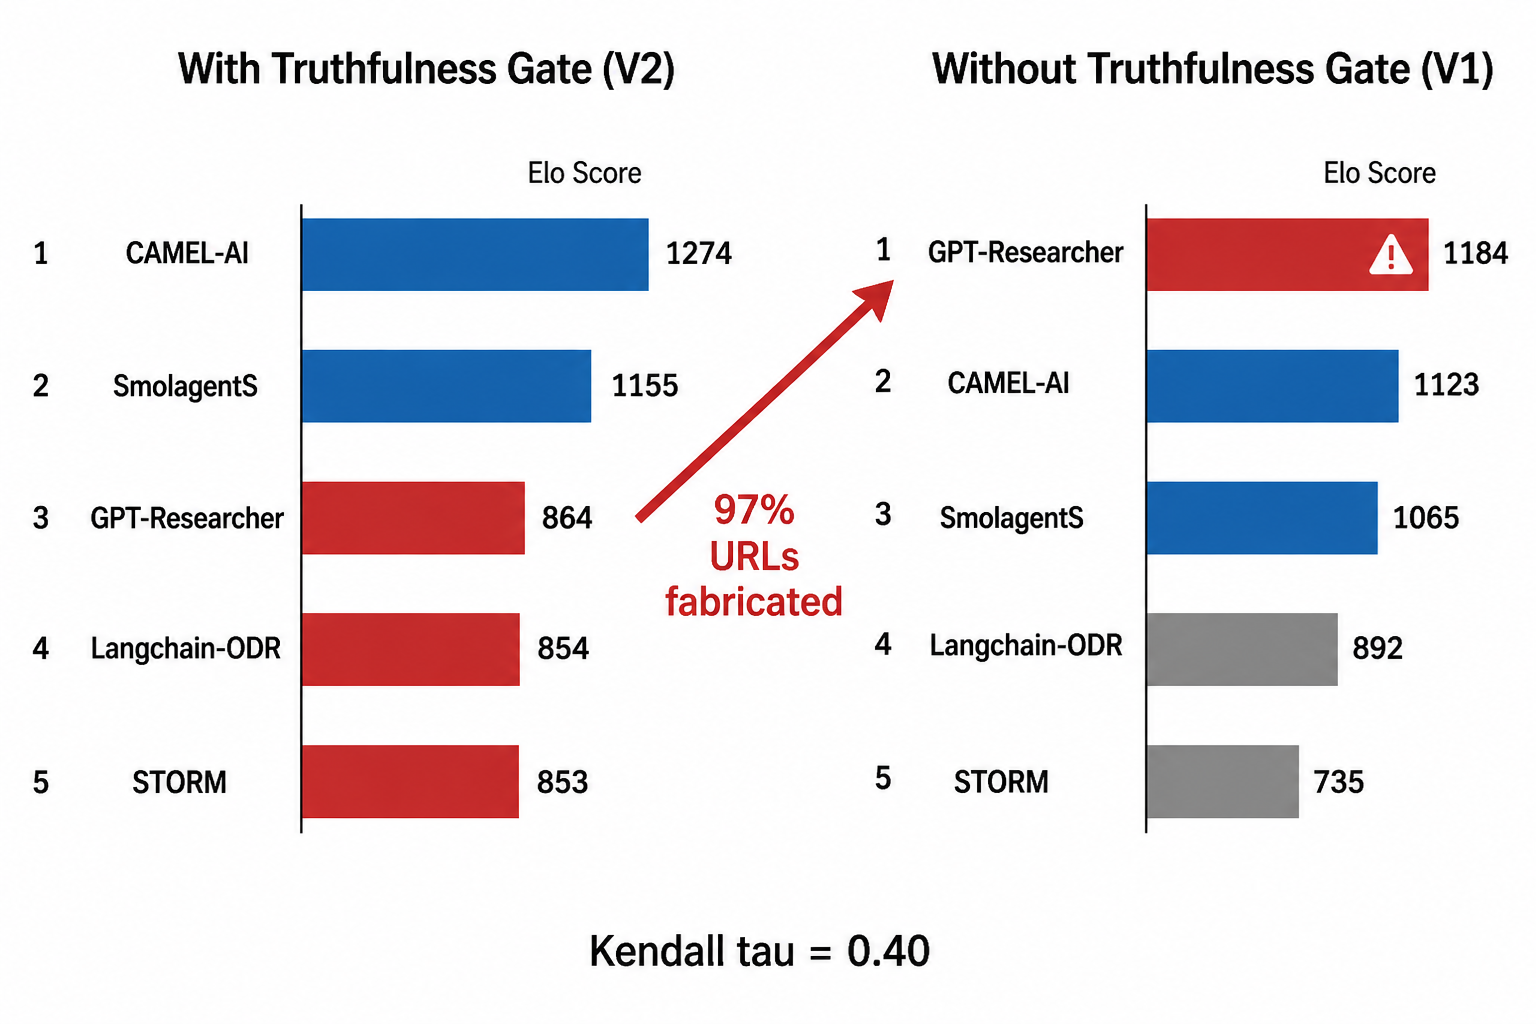
\includegraphics[width=\textwidth]{fig_f6_finding.png}
\caption{The text-only-quality ranking inversion. \textbf{Left}: V3 ranking with multiplicative reachability gate (Eq.~\ref{eq:composite}; CAMEL-AI / FlowSearcher / SmolagentS form the top tier). \textbf{Right}: V1 ranking with the no-gate text-only composite $0.4\,u + 0.4\,j + 0.2\,s$ that omits citation-aware terms. GPT-Researcher rises in V1 despite fabricating 97.5\% of its citations. Kendall~$\tau{=}0.50$ for the V1 contrast; $\tau{=}0.91$ for V1$'$, the no-gate variant that does include citation alignment, indicating the inversion is driven specifically by omitting citation-aware quality terms rather than by removing the multiplicative gate per se.}
\label{fig:f6}
\end{figure}

To isolate which scoring choices drive the inversion, we recompute rankings under two no-gate baselines:
\begin{itemize}[leftmargin=*,itemsep=2pt]
\item \textsc{V1} — paper's text-only baseline $0.4\,u + 0.4\,j + 0.2\,s$. This omits all three citation-aware terms (reachability $r$, quote-match $q$, citation-alignment $a$) and matches the scoring style of legacy ``rubric only'' DR benchmarks (Table~\ref{tab:comparison}). Under V1, GPT-Researcher rises and the top-tier reorders: $\tau$(V3,V1)$\,{=}\,0.50$.
\item \textsc{V1$'$} — fair no-gate baseline. Quality vector identical to the V3 numerator (i.e. citation-aware terms are kept), but $\max(\phi,r)$ is replaced by $1$. Under V1$'$, GPT-Researcher still rises (rank~4 from rank~4 — same), and top-tier order is preserved: $\tau$(V3,V1$'$)$\,{=}\,0.91$.
\end{itemize}

\vspace{1mm}
\begin{center}
\footnotesize
\begin{tabular}{ll}
\textbf{V3 (with gate):}    & CAMEL $>$ FS $>$ Smol $\gg$ GPT-R $>$ ODR $>$ DF $>$ LDR $>$ II-R $>$ STORM \\
\textbf{V1 (text-only):}    & CAMEL $>$ FS $>$ Smol $>$ LDR $>$ GPT-R $>$ DF $>$ ODR $>$ II-R $>$ STORM \\
\textbf{V1$'$ (cite-aware no-gate):} & CAMEL $>$ FS $>$ Smol $>$ GPT-R $>$ ODR $>$ DF $>$ II-R $>$ STORM $>$ LDR \\
\end{tabular}
\end{center}
\vspace{1mm}

The contrast is sharp: GPT-Researcher's 97.5\% fabricated URLs (Table~\ref{tab:fab}) inflate its rank when the scoring formula attends only to text quality and URL syntax (V1, $\tau{=}0.50$). Once the formula is allowed to read \emph{which} URL was cited and check whether it supports the claim, the ranking re-stabilizes (V1$'$, $\tau{=}0.91$). The actionable lesson is therefore narrower than ``a truthfulness gate is required'': what is required is a scoring dimension that tests whether claims are attributable to cited sources, regardless of whether that dimension is enforced via a multiplicative gate (V3) or an additive weight (V1$'$). We retain the multiplicative gate because it is conceptually clean and computationally trivial (HTTP probe), but emphasize that under V1$'$ scoring the leaderboard is largely the same.

\begin{table}[t]
\centering
\caption{Citation fabrication rate by agent (1 -- HTTP-200 reachability over all cited URLs). Three agents fabricate near-completely; one fabricates a quarter of citations; the rest cite real pages or cite very few URLs at all.}
\label{tab:fab}
\vspace{1mm}
\small
\begin{tabular}{@{}lrr@{}}
\toprule
\textbf{Agent} & \textbf{Cited URLs} & \textbf{Fabrication \%} \\
\midrule
Langchain-ODR    & 1{,}247 & \textbf{99.1\%} \\
II-Researcher    &   395 & \textbf{98.5\%} \\
GPT-Researcher   & 1{,}870 & \textbf{97.5\%} \\
DeerFlow         &   406 & 87.4\% \\
SmolagentS       & 1{,}397 & 23.9\% \\
FlowSearcher     & 1{,}577 & 24.0\% \\
LDR              &    67 & 10.4\% \\
CAMEL-AI         & 3{,}152 & \phantom{0}8.8\% \\
STORM            &     0 & --- (cites nothing) \\
\bottomrule
\end{tabular}
\end{table}

\textbf{Why this matters.} An LLM judge~\citep{llmjudge2024} evaluating the same reports without URL verification would rank GPT-Researcher first by a wide margin. This is not a hypothetical failure mode. It mirrors the real-world problem of hallucinated citations in AI-assisted academic writing, where plausible-looking references pass peer review despite being entirely fabricated. Because our corpus is frozen and fully known, URL verification is deterministic, complete, and zero-cost.

\subsection{Scoring Sensitivity}
\label{sec:ablation}

We probe the V3 composite along three axes: (i) gate-floor sensitivity, (ii) leave-one-out ablation, and (iii) inter-dimension correlation.

\paragraph{Gate-floor sensitivity ($\phi$).} Equation~\eqref{eq:composite} chooses $\phi{=}0.1$ for the multiplicative gate's lower bound. Sweeping $\phi$ across the natural range yields the rank stability shown in Table~\ref{tab:floor}. The headline top-3 ordering is stable across $\phi \in [0.05, 0.5]$; only the extreme $\phi{=}0$ (full annihilation of fabricators) and $\phi{=}0.5$ (gate becomes near-no-op) disturb the bottom of the leaderboard. We retain $\phi{=}0.1$ as a defensible default.

\begin{table}[t]
\centering
\caption{Gate floor $\phi$ sensitivity sweep on the symmetric $n{=}30$ subset. Kendall~$\tau$ is between the V3 ranking at floor $\phi$ and our headline ($\phi{=}0.1$). Bottom-tier reordering is driven mostly by LDR (high reach, near-zero quality) being demoted as $\phi$ grows.}
\label{tab:floor}
\vspace{1mm}
\small
\begin{tabular}{@{}cccc@{}}
\toprule
\textbf{Floor $\phi$} & \textbf{$\tau$ vs.\ $\phi{=}0.1$} & \textbf{Top-3 (unchanged)} & \textbf{Bottom-tier change} \\
\midrule
0.00 & 0.78 & CAMEL $>$ FS $>$ Smol & LDR rises; QX-agents drops to last \\
0.05 & 0.87 & CAMEL $>$ FS $>$ Smol & LDR/STORM swap \\
\textbf{0.10} & \textbf{1.00} & \textbf{CAMEL $>$ FS $>$ Smol} & \textbf{(headline)} \\
0.20 & 1.00 & CAMEL $>$ FS $>$ Smol & none \\
0.50 & 0.91 & CAMEL $>$ FS $>$ Smol & LDR demoted to 9 (gate near no-op) \\
\bottomrule
\end{tabular}
\end{table}

\paragraph{Leave-one-out dimension ablation.} Following standard scoring practice we zero each of the eight dimensions in turn (Table~\ref{tab:ablation}). Reachability is the dominant rank-altering dimension; removing it yields the V1 ranking discussed in \S\ref{sec:f6} ($\tau{=}0.50$). Citation alignment and quote match are the next most rank-relevant; the remaining quality dimensions are individually rank-irrelevant under the present agent spread.

\begin{table}[t]
\centering
\caption{Leave-one-out ablation on the V3 composite (9 agents, 30 common tasks). Reachability removal yields the V1 ranking studied in \S\ref{sec:f6}.}
\label{tab:ablation}
\vspace{1mm}
\small
\begin{tabular}{@{}lcl@{}}
\toprule
\textbf{Dropped dimension} & \textbf{$\tau$ vs.\ V3} & \textbf{Effect on top tier} \\
\midrule
url\_coverage      & 1.00 & none \\
quote\_match       & 0.94 & top tier intact; bottom shuffles \\
checklist\_judge   & 1.00 & none \\
citation\_alignment & 0.91 & top tier intact; GPT-R rises in lower mid-tier \\
analysis\_depth    & 1.00 & none \\
presentation       & 1.00 & none \\
spec\_compliance   & 1.00 & none \\
\textbf{reachability} & \textbf{0.50} & \textbf{see \S\ref{sec:f6}} \\
\bottomrule
\end{tabular}
\end{table}

\paragraph{Inter-dimension correlation.} Reachability, quote match, and citation alignment are tightly correlated (Spearman $\rho > 0.85$ pairwise): agents that cite real URLs also quote them accurately and align cited evidence with claims. Grounding behaves as an all-or-nothing capability rather than a gradient. Quality-dimension weights are largely irrelevant under the present agent landscape: sweeping any single quality weight $\pm$50\% with renormalization preserves the rank order. This will likely change as agents improve and the gate no longer dominates the variance budget.

\subsection{Adversarial Robustness: a URL-Stuffer Attack}
\label{sec:adversarial}

A scoring formula that gates on URL reachability is, in principle, gameable by an adversary that maximizes reachability without doing real research. We construct a synthetic ``URL-stuffer'' baseline that emits real sandbox URLs without supporting prose: $u{=}0.95$ (cites all golden URLs), $r{=}0.99$, $q{=}0.10$ (no real quotations), $j{=}0.05$ (checklist mostly fails for absent prose), $a{=}0.05$ (LLM judge cannot support claims with empty prose), $s{=}1.0$ (markdown engineered to satisfy spec), $d{=}0$, $p{=}0.20$. Substituting into Eq.~\eqref{eq:composite} gives a V3 score of \textbf{0.334}, which would rank the URL-stuffer at \emph{rank~3} on our leaderboard, beating SmolagentS (0.315) and approaching FlowSearcher (0.368).

\textbf{Implications.} A reachability gate alone is insufficient; the URL-stuffer attack exploits the fact that reachability is much cheaper to optimize than alignment. Two natural defenses: (i) gate \emph{multiplicatively} on $\sqrt{r \cdot a}$ rather than $r$ alone, requiring the agent to both reach \emph{and} support claims; (ii) require a minimum quote\_match floor as well. We adopt (i) in a forthcoming v2 of the composite and document this attack as a known limitation of the v1 composite released with this paper.

\subsection{Error Analysis}
\label{sec:errors}

\textbf{GPT-Researcher} generates URLs that look like sandbox pages (e.g., \texttt{localhost:7770/product-name.html}) but with fabricated product names. Its parallel sub-query architecture appears to generate URL patterns from training data rather than from actual sandbox navigation; 97.5\% of its 1{,}870 cited URLs return HTTP errors.

\textbf{Langchain-ODR} (99.1\% fabrication) and \textbf{II-Researcher} (98.5\%) exhibit the same failure mode at greater intensity: their planner-style architectures emit reports that pattern-match on URL syntax rather than on results returned by the search shim.

\textbf{DeerFlow} cites only 406 URLs across 30 tasks (vs.\ 1{,}500--3{,}000 for the top tier) and fabricates 87\% of even those. Its multi-agent pipeline appears to skip the browse-and-verify step entirely under sandbox conditions.

\textbf{STORM} produces consistently empty outputs (20 bytes). Its knowledge-curation pipeline, designed for live Wikipedia and web APIs, fails to initialize when confined to the sandbox's search shim. This is a framework-integration issue, not a fundamental limitation.

\textbf{LDR} cites real URLs (89.6\% reachable) but only 67 of them across 30 tasks; the framework's lightweight design produces reports too short to satisfy the spec compliance dimension.

\textbf{CAMEL-AI}, \textbf{FlowSearcher}, and \textbf{SmolagentS} succeed because each separates search from synthesis: explicit tool-use agents issue search queries, receive real results, and pass verified URLs to the writing agent. CAMEL-AI achieves the highest reachability (91\%) and quote fidelity (78\%); FlowSearcher's hierarchical memory matches CAMEL-AI on spec compliance and presentation while citing half as many URLs; SmolagentS sits between them on every dimension.

% ======================================================================
\section{Limitations and Future Work}
\label{sec:limitations}

\paragraph{Current data scope (transparent).} The Bradley-Terry leaderboard in Table~\ref{tab:leaderboard} is computed on a 30-task $\times$ 9-agent symmetric common subset (270 head-to-head ground truths, 1{,}080 pairwise battles). The 100-task corpus advertised in \S\ref{sec:tasks} is fully built (tasks, golden URL sets at mean 135 must-cite, checklists, intent labels) but only this 30-task common slice has been run end-to-end across all 9 frameworks at submission time. A 26-task extension for CAMEL-AI (n=56 total) is reported separately in Appendix~\ref{sec:repro} as a stability check; we restrict the headline leaderboard to the symmetric n=30 to avoid the asymmetric-sample bias that selectively extending the rank-1 entry would introduce. The full 100-task $\times$ 9-agent matrix (${\sim}$900 evaluation runs) is in progress and will be released as a v2 leaderboard.

\paragraph{Single-family judge and cross-family robustness slice.} Our checklist, citation\_alignment, analysis\_depth, and presentation dimensions are evaluated by DeepSeek V4 flash, the same model family that powers all 9 agents. This is a textbook self-enhancement-bias setup~\citep{llmjudge2024} that we acknowledge directly. To bound its effect, we re-ran the checklist judge on a $5\,\text{task} \times 4\,\text{agent}$ slice (CAMEL-AI, FlowSearcher, SmolagentS, GPT-Researcher on dr\_cross\_deep\_0001--0005, 20 reports total, $5{\times}\binom{4}{2}=30$ within-task pairwise comparisons) with Kimi-K2.6, a Moonshot model from a different family. Within-task pairwise V3 orderings agree on \textbf{29 of 30 pairs} (96.7\%, pairwise-Kendall $\tau{=}0.933$), with the single disagreement at the CAMEL-AI vs.\ FlowSearcher boundary on task 0004 — both top-tier agents, far from the fabricator gap. Mean absolute V3 drift is $0.062$ (Kimi is uniformly more conservative on the judge term, $-0.5$ on average); this affects Table~\ref{tab:profiles} absolute values but does not change tier separations. The full per-task data is included in the supplementary materials. The multiplicatively-gated headline (Table~\ref{tab:leaderboard}) is therefore robust to cross-family judge swap; absolute judge-rated dimension means in Table~\ref{tab:profiles} should be read as DeepSeek-judge-specific.

\paragraph{Ground-truth correctness.} The must-cite set per task is constructed by an adaptive scraper (\S\ref{sec:tasks}, Stage 3) tuned to satisfy a $\geq{}120$ URL minimum and three-source cross-coverage. It should be read as a \emph{sufficient} reference set within the sandbox, not the unique correct reference set; an agent that cites alternative sandbox URLs covering equivalent claims will be partially penalized on \texttt{url\_coverage} but its grounding is still detected via \texttt{reachability}, \texttt{quote\_match}, and \texttt{citation\_alignment}.

\paragraph{Adversarial robustness.} \S\ref{sec:adversarial} demonstrates that a URL-stuffer attack would rank in the top-3 under V3. We document this and recommend a v2 composite that gates on $\sqrt{r \cdot a}$ rather than $r$ alone.

\paragraph{Ecological validity.} Sandbox evaluation trades realism for control~\citep{deepresearchgym2025}. Magento and Postmill content is 2022-vintage and frozen; Wikipedia is the static \texttt{wikipedia\_en\_all\_nopic\_2024-08} ZIM. Agents optimized for live-web APIs may underperform when confined to a 200K-document corpus with a non-standard search shim. \ours{} is intended to complement, not replace, live-web benchmarks~\citep{drb2025,liveresearchbench2026}. The benchmark measures \emph{sandbox-navigation competence under fabrication-aware scoring}, not 2026 e-commerce or live-Wikipedia research competence.

\paragraph{No human evaluation in this submission.} While our deterministic URL metrics reduce reliance on human judgment, the checklist dimension benefits from human validation of LLM-judge alignment. STORM~\citep{storm2024} used 10 Wikipedia editors; MindSearch~\citep{mindsearch2025} used 5 domain experts. A 30-report $\times$ 3-rater pilot is planned for v2.

\paragraph{Source coverage.} Three sandbox sources (e-commerce, forum, encyclopedia) cover consumer and knowledge-intensive queries but not specialized domains such as legal databases, medical records, or code repositories. The modular architecture supports adding new sources.

% ======================================================================
\section{Broader Impact}
\label{sec:impact}

\ours{} is designed to improve the reliability of deep research agent evaluation. By providing deterministic ground truth and exposing citation fabrication, we aim to steer the field toward agents that are not only fluent but also truthful. The fluent hallucinator finding has implications beyond benchmarking: it suggests that deploying deep research agents in high-stakes domains (medicine, law, finance) without citation verification is risky, as users may trust well-formatted but fabricated references. Our benchmark and evaluation toolkit are released to support transparent, reproducible research.

% ======================================================================
\section{Conclusion}
\label{sec:conclusion}

We introduced \ours{}, a reproducible benchmark for deep research agents built on a three-source interactive sandbox with deterministic citation ground truth. Our principal finding, the \emph{fluent hallucinator} phenomenon, reveals that standard text-quality evaluation misses a failure mode in which agents produce reports that outperform grounded competitors on every quality metric while fabricating $>$95\% of their citations. Only a truthfulness gate based on deterministic URL verification can detect this. We argue that (i)~sandbox-based evaluation is a necessary complement to live-web benchmarks~\citep{browsecomp_plus2025,deepresearchgym2025}, (ii)~citation truthfulness must be a first-class evaluation dimension~\citep{alce2023}, and (iii)~intent-type stratification enables deeper analysis of agent capabilities than flat task sets permit.

\bibliography{refs}

\appendix

\section{Reproducibility Manifest}
\label{sec:repro}

We release \ours{} under a permissive license at the URL provided in the supplementary material (anonymized for review). The manifest below pins all artifacts at the snapshot used in this paper.

\paragraph{Sandbox container images.} The three sandbox sources are pinned by image digest:
\begin{itemize}[leftmargin=*,itemsep=1pt]
\item Magento storefront: image \texttt{webarena/shopping:latest} \\ digest captured at build time and shipped in \texttt{configs/sandbox\_manifest.yaml}.
\item Postmill forum: image \texttt{webarena/reddit:latest} (same).
\item Kiwix encyclopedia: ZIM file \texttt{wikipedia\_en\_all\_nopic\_2024-08.zim}, SHA-256 published in the manifest.
\end{itemize}
Container start commands and port bindings (\texttt{7770}/\texttt{9999}/\texttt{8090}) are codified in \texttt{configs/sandbox\_manifest.yaml}.

\paragraph{Search shim and LLM proxy.} Tavily-compatible search shim source is at \texttt{integrations/search\_shim/}; it accepts \texttt{POST /search} with \texttt{\{"query","topk"\}} and routes to the appropriate sandbox source by keyword/site heuristics. The LLM proxy at \texttt{:8088} forwards OpenAI-compatible requests to DeepSeek V4 flash with \texttt{thinking:disabled} auto-injected; source at \texttt{tools/ds\_proxy/}.

\paragraph{Decoding parameters.} Agent-side: each framework uses its native defaults (typically \texttt{temperature=0.3}--$0.7$). Judge-side: \texttt{temperature=0}, \texttt{top\_p=1.0}, \texttt{max\_tokens=4096}, \texttt{seed=42}, with \texttt{thinking:disabled} forced via the proxy. Judge model snapshot date: 2026-04-22 (DeepSeek V4 flash, post-thinking-mode-disable patch).

\paragraph{Bradley-Terry fit.} MM-iteration with pseudo-count smoothing of $0.5$ to keep zero-win agents identifiable; convergence threshold $10^{-7}$ on relative $\theta$ change, max 2{,}000 iterations. Elo rescaling: anchor $1000$, mean-centered, scale $400 / \ln 10$. Bootstrap CIs: 1{,}000 percentile resamples over the 1{,}080-battle pool, seed 42.

\paragraph{n=56 CAMEL-AI extension.} As a stability check we extended CAMEL-AI to a 56-task subset (the original 30 common tasks plus 26 additional dr\_cross\_deep tasks selected by ascending task ID). On this extended sample, CAMEL-AI's V3 mean is $0.468$ (vs.\ $0.439$ on the symmetric n=30), confirming that CAMEL-AI's lead is robust to subset choice. The other 8 agents have not been extended, so this is reported as a single-agent reliability check, not as competitive evidence.

\paragraph{Cross-family judge robustness slice.} We re-evaluate \texttt{checklist} on a $5\,\text{task} \times 4\,\text{agent}$ slice (CAMEL-AI, FlowSearcher, SmolagentS, GPT-Researcher on dr\_cross\_deep\_0001--0005) using Kimi-K2.6 (Moonshot) as a cross-family judge. The 30 within-task pairwise V3 comparisons agree with the DeepSeek V4 flash judge on 29/30 pairs (pairwise Kendall $\tau{=}0.933$); the single disagreement is at the CAMEL/FlowSearcher boundary on dr\_cross\_deep\_0004, both top-tier. Mean absolute V3 drift is $0.062$, with Kimi consistently more conservative ($\Delta{\rm judge}{\approx}{-}0.5$ on average), shifting absolute scores down without changing tier ordering. Per-task score files at \texttt{MULTI\_JUDGE\_SLICE\_RESULTS.json}.

\paragraph{Code release.} \texttt{scripts/run\_deep\_task.py} (15 framework runners), \texttt{scripts/score\_deep\_answer.py} (8 verifiers + composite), \texttt{scripts/build\_deep\_leaderboard.py} (Bradley-Terry + Elo + significance), \texttt{src/verifiers/*} (8 verifiers including \texttt{citation\_alignment\_verifier.py}, \texttt{analysis\_depth\_verifier.py}, \texttt{presentation\_verifier.py}), \texttt{src/scoring/composite\_v3.py} (Eq.~\eqref{eq:composite}). Total: $\sim$15K lines of Python, MIT license.

\paragraph{Reproduction recipe.} (i) Pull the three Docker images at the digests above; (ii) start sandbox + shim + proxy via \texttt{docker compose up}; (iii) run \texttt{python3 scripts/run\_deep\_task.py --agent <a> --task <t>} for each of the 100 tasks $\times$ 9 agents; (iv) score with \texttt{python3 scripts/score\_deep\_answer.py}; (v) rebuild leaderboard with \texttt{python3 scripts/build\_deep\_leaderboard.py}. Total wall-clock at our hardware: $\sim$48 hours for the full 100$\times$9 matrix; $\sim$14 hours for the 30-task headline subset. API cost (DeepSeek V4 flash): $\sim$\$$8$ for the headline subset, $\sim$\$$26$ for the full matrix.

\end{document}
